%%%%%%%%%%%%%%%%%%%%%% CHAPTER ONE %%%%%%%%%%%%%%%%%%%%%%%%%%%%%%%%%%%%%%%
\chapter{Installing Rocks}

\section{Rocks Installation}
We advise you to go through the rocks official \cite{rocksinstall} documentation  before the installation to understand the basic principles of clusters.\\
%Please refer to Appendix I for detailed steps.
\subsection{Physical Assembly}
The first thing to manage is the physical deployment of a cluster.The following diagram shows how the frontend and compute nodes must be connected:

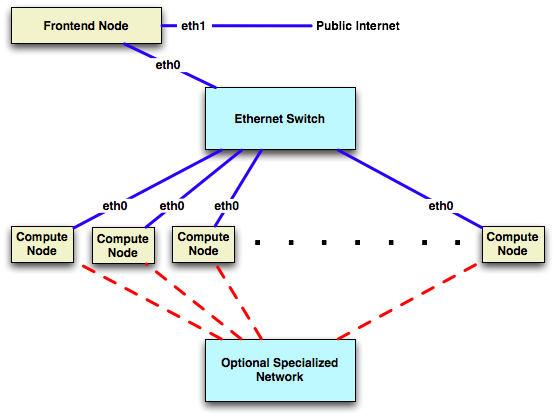
\includegraphics[scale=.5]{cluster.png} 
\paragraph{}
On the Compute nodes (Vm-container), the Ethernet interface that Linux maps to eth0 should be connected to the cluster's Ethernet switch. This network is considered private, i.e, all traffic on this network is physically separated from the external public network (e.g., The Internet).
On the Frontend, at least two Ethernet interfaces are required. The interface that Linux maps to eth0 should be connected to the same Ethernet network as the compute nodes. The interface that Linux maps to eth1 should be connected to the external network (Internet or your organization's intranet).
\paragraph{}
In our case the eth0 is connected to the switch placed within the rack and eth1 of the Frontend is connected to public network under Networks systems lab’s subnet.

\section{Frontend Installation}
The installation on the Frontend is done using a disk image either by a DVD or a bootable USB drive.The Jumbo DVD has all the required rolls in one single disk image. The x86 64 version of Rocks 6.1 can be downloaded from here \cite{rocksdownload}

\begin{itemize}
\item Insert the DVD/USB Drive and restart the main node (Frontend). A boot screen will be displayed with a prompt. Enter the following command to start the installation: 
 \item The next screen shows the list of all rolls in the DVD. Select the required rolls from the list. The Kernel, Base, OS and Web-Server rolls are mandatory. Additional rolls can be installed by using DVD based rolls. Hit next to proceed.
\item The next screen is for entering Cluster Information. Enter the details for Host name, cluster name, organization, locality, state, country, contact, URL, latitude and longitude. The fully-qualified host name is mandatory and is important for several cluster services.
 \item The next screen has the option to set the eth1 ( which is the interface to public network ) IP address. This is the public IP of the cluster(connected to the internet). Enter the public IP as 192.168.41.203.
 
\item The next screen has the option to set the private network eth0 IP address and netmask. This is the IP address of the private network between the Frontend and the nodes. The IP address used is 10.1.1.1 and the netmask is 255.255.0.0.

\item Now configure the gateway and DNS. Gateway used is 192.168.41.1 and DNS servers used are 192.168.254.2, 192.168.254.3.

\item Enter the root password of the cluster when prompted.
\item Configure the time by selecting the time zone for the cluster followed by inputting a Network Time Protocol(NTP) server that will keep the clock on the frontend in sync.

\item The next screen shows the option for the partitioning of the hard disk of the Frontend. Select "Manual Partitioning" since the configuration of " Auto Partitioning provides insufficient space for the /var partition which is used by the Eucalyptus Cloud to upload Virtual Machine Images.

\item The partition used for frontend is: \\ 
\end{itemize}

\begin{center}
\begin{tabular}{ | l | c | r |}
    \hline
    Partition Name & Size  \\ \hline
    /&170GB \\ 
    /var&480GB \\
	/export&170GB \\
	swap&1GB    \\
    \hline
  \end{tabular}
\end{center}
%%%%%%%%%%%%%%%%%%%%%% END OF CHAPTER ONE %%%%%%%%%%%%%%%%%%%%%%%%%%%%%%%%%%%%%%%

%%%%%%%%%%%%%%%%%%%%%CHAPTER 2 INTRO TO EUCA%%%%%%%%%%%%%%%%%%%%%%%%%%%%%%%%%%%%%
\chapter{Introduction to Eucalyptus}

Eucalyptus is a Linux-based software architecture that implements scalable private and hybrid clouds within your existing IT infrastructure. Eucalyptus allows you to provision your own collections of resources (hardware, storage, and network) using a self-service interface on an as-needed basis. \linebreak
\\
You deploy a Eucalyptus cloud across your enterprise’s on-premise data center. Users access Eucalyptus over your enterprise's intranet. This allows sensitive data to remain secure from external intrusion behind the enterprise firewall.
\linebreak

You can install Eucalyptus on the following Linux distributions:
\begin{itemize}
\item CentOS 6
\item Red Hat Enterprise Linux 6
\end{itemize}

\section{Overview}
Eucalyptus was designed to be easy to install and as non-intrusive as possible. The software framework is modular, with industry-standard, language-agnostic communication. Eucalyptus provides a virtual network overlay that both isolates network traffic of different users and allows two or more clusters to appear to belong to the same Local Area Network (LAN). Also, Eucalyptus offers API compatibility with Amazon’s EC2, S3, and IAM services. This offers you the capability of a hybrid cloud.

\section{Eucalyptus Components}
Eucalyptus is comprised of six components: Cloud Controller (CLC), Walrus, Cluster Controller (CC), Storage Controller (SC), Node Controller (NC) and an optional VMware Broker (Broker or VB). Other than the VMware Broker, each component is a stand-alone web service. This architecture allows Eucalyptus both to expose each web service as a well-defined, language-agnostic API, and to support existing web service standards for secure communication between its components.
A detailed description of each Eucalyptus component follows.\linebreak
\subsection{Cloud Controller}
The Cloud Controller (CLC) is the entry-point into the cloud for administrators, developers, project managers, and end-users. The CLC queries other components for information about resources, makes high-level scheduling decisions, and makes requests to the Cluster Controllers (CCs). As the interface to the management platform, the CLC is responsible for exposing and managing the underlying virtualized resources (servers, network, and storage). You can access the CLC through command line tools that are compatible with Amazon’s Elastic Compute Cloud (EC2) and through a web-based Eucalyptus Administrator Console.
\subsection{Walrus}
Walrus allows users to store persistent data, organized as buckets and objects. You can use Walrus to create, delete, and list buckets, or to put, get, and delete objects, or to set access control policies. Walrus is interface compatible with Amazon’s Simple Storage Service (S3), providing a mechanism for storing and accessing virtual machine images and user data. Walrus can be accessed by end-users, whether the user is running a client from outside the cloud or from a virtual machine instance running inside the cloud.
\subsection{Cluster Controller}
The Cluster Controller (CC) generally executes on a machine that has network connectivity to both the machines running the Node Controllers (NCs) and to the machine running the CLC. CCs gather information about a set of NCs and schedules virtual machine (VM) execution on specific NCs. The CC also manages the virtual machine networks. All NCs associated with a single CC must be in the same subnet.
\subsection{Storage Controller}
The Storage Controller (SC) provides functionality similar to the Amazon Elastic Block Store (Amazon EBS). The SC is capable of interfacing with various storage systems. Elastic block storage exports storage volumes that can be attached by a VM and mounted or accessed as a raw block device. EBS volumes persist past VM termination and are commonly used to store persistent data. An EBS volume cannot be shared between VMs and can only be accessed within the same availability zone in which the VM is running. Users can create snapshots from EBS volumes. Snapshots are stored in Walrus and made available across availability zones. Eucalyptus with SAN support lets you use your enterprise-grade SAN devices to host EBS storage within a Eucalyptus cloud.
\subsection{Node Controller}
The Node Controller (NC) executes on any machine that hosts VM instances. The NC controls VM activities, including the execution, inspection, and termination of VM instances. It also fetches and maintains a local cache of instance images, and it queries and controls the system software (host OS and the hypervisor) in response to queries and control requests from the CC. The NC is also responsible for the management of the virtual network endpoint.
\section{Understanding the Eucalyptus Architecture}
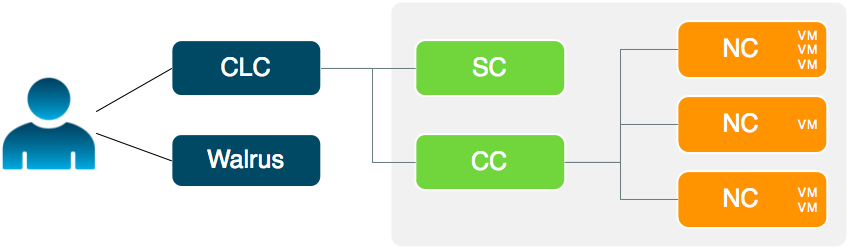
\includegraphics[scale=0.75]{euca-arch.png} 
\linebreak
The cloud components, Cloud Controller (CLC) and Walrus, communicate with cluster components, the Cluster Controllers (CCs) and Storage Controllers (SCs). The CCs and SCs, in turn, communicate with the Node Controllers (NCs). The networks between machines hosting these components must be able to allow TCP connections between them.
\\ \\
However, if the CCs are on separate network interfaces (one for the network on which the cloud components are hosted and another for the network that NCs use) the CCs will act as software routers between these networks in some networking configurations. So each cluster can use an internal private network for its NCs and the CCs will route traffic from that network to a network shared by the cloud components.
\\ \\
Virtual machines (VMs) run on the machines that host NCs. You can use the CCs as software routers for traffic between clients outside Eucalyptus and VMs. Or the VMs can use the routing framework already in place without CC software routers. However, depending on the layer-2 isolation characteristics of your existing network, you might not be able to implement all of the security features supported by Eucalyptus. 
\\ \\
Note : In our cluster we have installed CC, Walrus, CLC, SC in the frontend and the NC’s in the nodes.
%%%%%%%%%%%%%%%%%%%%%%%%%END OF CHAPTER 2%%%%%%%%%%%%%%%%%%%%%%%%%%%%%%%%%%%%%%%%%%%%%%%%%%%%%%%%%%%



%%%%%%%%%%%%%%%%%%%%%% CHAPTER Three %%%%%%%%%%%%%%%%%%%%%%%%%%%%%%%%%%%%%%%

\chapter{Network Configuration}

\section{Introduction}
This is the most intriguing part of cloud installation, where we will have to decide upon a networking mode available in Eucalyptus. For Zeus cloud we are using Managed (No VLAN) Mode. Read more about managed no vlan here\cite{managednovlan}.

\subsection{Enabling Public Web Access to Your Frontend}

To permanently enable selected web access to the cluster from other machines on the public network, follow the steps below. Apache's access control directives will provide protection for the most sensitive parts of the cluster web site, however some effort will be necessary to make effective use of them.

To open port 80 (the 'www' service) for the public network of frontend,  execute:

\begin{lstlisting}[language=bash]
rocks open host firewall localhost \
network=public protocol=tcp service=www
\end{lstlisting}
Now you can try accessing the ip \url{192.168.41.203} or uri \url{zeus.nitc.ac.in}over network to view the rocks cluster web frontend.

\subsection{Configuring Firewall}

Eucalyptus components use a variety of ports to communicate. The following table lists the all of the important ports used by Eucalyptus.

\begin{center}
\begin{tabular}{ | l | c | r |}
    \hline
Port&Description \\
TCP 8443& SSL port for the administrative web user interface. Configurable with euca-modify-property.\\
TCP 8772&DEBUG ONLY\\: JMX port. This is disabled by default, and can be enabled with the \-\-debug or \-\-jmx options for CLOUD\_OPTS. \\
TCP 8773&Web services port for the CLC, Walrus, SC, and VB; also used for external and internal communications by the CLC and Walrus. Configurable with euca-modify-property.\\
TCP 8774&Web services port on the CC. Configured in the eucalyptus.conf configuration file.\\
TCP 8775&Web services port on the NC. Configured in the eucalyptus.conf configuration file.\\
TCP 8776&Used by the image cacher on the CC. Configured in the eucalyptus.conf configuration file.\\
TCP 8777&Database port on the CLC.\\
TCP 8080&Port for the administrative web user interface. Forwards to 8443. Configurable with euca-modify-property.\\
UDP 7500&Distributed cache port on the CLC, Walrus, SC, and VB.\\
UDP 8773&HA membership port.\\
TCP/UDP 53&DNS port on the CLC.\\
\end{tabular}
\end{center}

\subsection{To open the required ports,run the following commands}
Here we are trying to open ports for Eucalyptus to communicate between its components, rocks command \emph{rocks add firewall} can be used to add firewall rules. 

Read the following rocks manual to understand more Managing firewall through Rocks \cite{mfirewal}.

\subsection{Opening ports in Frontend}
\begin{lstlisting}[language=bash]
rocks add firewall host=frontend network=public protocol=tcp service=8443 \ chain=INPUT action=ACCEPT rulename=E10-PORT-8443

rocks add firewall host=frontend network=public protocol=tcp service=8772 \
chain=INPUT action=ACCEPT rulename=E10-PORT-8772

rocks add firewall host=frontend network=public protocol=tcp service=8773 \
 chain=INPUT action=ACCEPT rulename=E10-PORT-8773

rocks add firewall host=frontend network=public protocol=tcp service=8774 \ 
chain=INPUT action=ACCEPT rulename=E10-PORT-8774

rocks add firewall host=frontend network=public protocol=tcp service=8776 \ 
chain=INPUT action=ACCEPT rulename=E10-PORT-8776

rocks add firewall host=frontend network=public protocol=tcp service=8777 \ 
chain=INPUT action=ACCEPT rulename=E10-PORT-8777

rocks add firewall host=frontend network=public protocol=tcp service=8080 \
chain=INPUT action=ACCEPT rulename=E10-PORT-8080

rocks add firewall host=frontend network=public protocol=tcp service=5005 \
chain=INPUT action=ACCEPT rulename=E10-PORT-5005

rocks add firewall host=frontend network=public protocol=udp service=7500 \
chain=INPUT action=ACCEPT rulename=E10-PORT-7500
\end{lstlisting}


Before synchronising the firewall rules we need to remove two rules from the existing firewall.
The command to remove the rules are 
\begin{lstlisting}[language=bash]
rocks remove firewall global rulename=R900-PRIVILEGED-TCP
rocks remove firewall global rulename=R900-PRIVILEGED-UDP
\end{lstlisting}
\subsection{Opening Web Access to Public}
Remove the rule which restrict the web access only to subnet 192.168.41.0/24
\begin{lstlisting}[language=bash]
rocks remove firewall host=localhost rulename=A40-WWW-PUBLIC-LAN
\end{lstlisting}

\subsection{Now, make it available to public}
\begin{lstlisting}[language=bash]
rocks add firewall host=frontend network=public protocol=tcp \
service=www chain=INPUT action=ACCEPT \
flags="-m state --state NEW --source 0.0.0.0/0.0.0.0" \
rulename=A40-WWW-PUBLIC-NEW
\end{lstlisting}
\subsection{Sync the above firewall rules to rocks frontend using }
\begin{lstlisting}[language=bash]
rocks sync host firewall frontend
\end{lstlisting}
\subsection{Accepting everything from TCP and UDP }
\begin{lstlisting}[language=bash]
iptables -A INPUT -p udp --dport 0:1023 -j ACCEPT
iptables -A INPUT -p tcp --dport 0:1023 -j ACCEPT
/sbin/service iptables save
\end{lstlisting}
\subsection{Opening ports required for DNS functioning}

\begin{lstlisting}[language=bash]
iptables -A INPUT -p tcp -m tcp --sport 53 --dport 1024:65535 -m state \ --state ESTABLISHED -j ACCEPT
iptables -A INPUT -p udp -m udp --sport 53 --dport 1024:65535 -m state \ --state ESTABLISHED -j ACCEPT
iptables -A OUTPUT -p tcp -m tcp --sport 1024:65535 --dport 53 -m state \ --state NEW,ESTABLISHED -j ACCEPT
iptables -A OUTPUT -p udp -m udp --sport 1024:65535 --dport 53 -m state \ --state NEW,ESTABLISHED -j ACCEPT
/sbin/service iptables save

\end{lstlisting}
\subsection{Opening ports in nodes}
Opening the web service in nodes
\begin{lstlisting}[language=bash]
rocks add firewall appliance=vm-container protocol=tcp \
service=8775 network=all chain=INPUT action=ACCEPT \
rulename=E10-PORT-8775
\end{lstlisting}
\subsection{Sync the firewall rules to all the nodes using }
\begin{lstlisting}[language=bash]
rocks sync host firewall vm-container
\end{lstlisting}
\section{Verify TCP/IP Connectivity}

Verify connectivity between the machines you’ll be installing Eucalyptus on. Some Linux distributions provide default TCP/IP firewalling rules that limit network access to machines. Disable these default firewall settings before you install Eucalyptus components to ensure that the components can communicate with one another.
Verify component connectivity by performing the following checks on the machines that will be running the listed Eucalyptus components.
\begin{enumerate}
\item Verify connection from and end-user to the CLC on ports 8773 and 8443
\item Verify connection from an end-user to Walrus on port 8773
\item Verify connection from the CLC, SC, and NC to Walrus on port 8773
\item Verify connection from Walrus, SC, and VB to CLC on port 8777
\item Verify connection from CLC to CC on port 8774
\item Verify connection from CC to VB on port 8773
\item Verify connection from CC to NC on port 8775
\item Verify connection from NC (or VB) to Walrus on port 8773 or you can verify the connection from the CC to Walrus on port 8773, and from an NC to the CC on port 8776
\item Verify connection from public IP addresses of Eucalyptus instances (metadata) and CC to CLC on port 8773
\item Verify TCP connectivity between CLC, Walrus, SC and VB
\item Verify connection between CLC, Walrus, SC, and VB on UDP ports 7500 and 8773

\end{enumerate}
We will use the program given below as socket which will  listen to specified a port (as a server ), run this program and telnet to the server's ip ( where you ran the program ) along with port number and check the connection.

\begin{lstlisting}[language=java]
import java.net.*;
import java.io.*;
public class PortMonitor {
    public static void main(String[] args) throws Exception {
         //Port to monitor
        final int myPort = Integer.parseInt(args[0]);
        ServerSocket ssock = new ServerSocket(myPort);
        System.out.println("port " + myPort + " opened");
         Socket sock = ssock.accept();
        System.out.println("Someone has made socket connection");
         OneConnection client = new OneConnection(sock);
        String s = client.getRequest();
     }
 }
class OneConnection {
    Socket sock;
    BufferedReader in = null;
    DataOutputStream out = null;
OneConnection(Socket sock) throws Exception {
        this.sock = sock;
        in = new BufferedReader(new InputStreamReader(sock.getInputStream()));
        out = new DataOutputStream(sock.getOutputStream());
    }
String getRequest() throws Exception {
        String s = null;
        while ((s = in.readLine()) != null) {
            System.out.println("got: " + s);
        }
        return s;
    }
}
\end{lstlisting}
Example 
( 1 ) Verify connection from and end-user to the CLC on ports 8773

Now run the program in frontend with argument 8773
\begin{lstlisting}[language=bash]
javac Portmonitor.java
java Portmonitor 8773
\end{lstlisting}
From any other system telnet into frontend with port 8773
\begin{lstlisting}[language=bash]
telnet 192.168.41.203 8773
Trying 192.168.41.203...
Connected to 192.168.41.203.
Escape character is '^]'.
hello
\end{lstlisting}
Output @ frontend when connection is established 
\begin{lstlisting}[language=bash]
port 8773 opened
Someone has made socket connection
got: hello
\end{lstlisting}
Understand the scenario for each of the verification step given above using the program and telnet.

\section{Configure SELinux}
SELinux is not supported by Eucalyptus
\begin{enumerate}
\item Open /etc/selinux/config and edit the line SELINUX=enforcing to SELINUX=permissive.
\item Save the file.
\item Run the following command: \\
\em{setenforce 0}
\end{enumerate}
\section{Configure NTP}

Eucalyptus requires that each machine have the Network Time Protocol (NTP) daemon started and configured to run automatically on reboot.
\linebreak
NTP in Frontend
\linebreak
Check the status of ntpd daemon 
\em{service ntpd status}
\linebreak
Update the time using any server
\em{ntpdate -u 0.pool.ntp.org}
\linebreak
Sync the time with the hardware clock 
\em{hwclock --systohc}
\linebreak
NTP in Nodes
\em{rocks run host vm-container "ntpd -u 0.pool.ntp.org ; hwclock --systohc"}

%%%%%%%%%%%%%%%%%%%%%% END OF CHAPTER THREE %%%%%%%%%%%%%%%%%%%%%%%%%%%%%%%%%%


%%%%%%%%%%%%%%%%%CHAPTER 4 IN THE MAKNIG%%%%%%%%%%%%%%%%%%%%%%%%%%%%%%%
\chapter{Installing Eucalyptus}
\subsection{Enable Centos Repo in frontend }
\begin{lstlisting}[language=bash]
sed i.backup 's/enabled = 0/enabled = 1/' /etc/yum.repos.d/CentOS-Base.repo
\end{lstlisting}
\subsection{Enable Centos Repo in Nodes }
\begin{lstlisting}[language=bash]
for i in {0..4}; do scp /etc/yum.repos.d/CentOS-Base.repo root@vm-container-0-$i:/etc/yum.repos.d/CentOS-Base.repo; done
\end{lstlisting} 
\subsection{Configure the Eucalyptus package repository} 
On Frontend:
\begin{lstlisting}[language=bash]
yum install http://downloads.eucalyptus.com/software/eucalyptus/3.3/centos/6/x86_64/eucalyptus-release-3.3.noarch.rpm 

sed -i.backup 's/enabled = 0/enabled = 1/' eucalyptus-release.repo 
\end{lstlisting} 
On the Nodes:
\begin{lstlisting}[language=bash]
for i in {0..4}; do scp /etc/yum.repos.d/euca2ools-release.repo root@vm-container-0-$i:/etc/yum.repos.d/euca2ools-release.repo ; done
\end{lstlisting}

\subsection{Configure the EPEL package repository}
On Frontend:
\begin{lstlisting}[language=bash]
yum install http://downloads.eucalyptus.com/software/eucalyptus/3.3/centos/6/x86_64/epel-release-6.noarch.rpm

sed -i.backup 's/enabled = 0/enabled = 1/' epel.repo
\end{lstlisting}

On the nodes:
\begin{lstlisting}[language=bash]
for i in {0..4}; do scp /etc/yum.repos.d/epel.repo root@vm-container-0-$i:/etc/yum.repos.d/epel.repo ; done
\end{lstlisting}

\subsection{Configure the ELRepo repository on frontend}
\begin{lstlisting}[language=bash]
yum install http://downloads.eucalyptus.com/software/eucalyptus/3.3/centos/6/x86_64/elrepo-release-6.noarch.rpm
sed -i.backup 's/enabled = 0/enabled = 1/' elrepo.repo
\end{lstlisting}

\subsection{Install the Eucalyptus node controller software on each planned NC host}
\begin{lstlisting}[language=bash]
rocks run host vm-container "yum install eucalyptus-nc"
\end{lstlisting}

Check that the KVM device node has proper permissions.
Run the following command:
\begin{lstlisting}[language=bash]
rocks run host vm-container "ls -l /dev/kvm"
\end{lstlisting}
Verify the output shows that the device node is owned by user root and group kvm.
\begin{lstlisting}[language=bash]
crw-rw-rw- 1 root kvm 10, 232 Nov 30 10:27 /dev/kvm
\end{lstlisting}

If your kvm device node does not have proper permissions, you need to reboot your node and change settings in BIOS to enable KVM.
\\ \linebreak
\subsection{Install the Eucalyptus cloud controller software on each planned CLC host}
\begin{lstlisting}[language=bash]
yum install eucalyptus-cloud
\end{lstlisting}
\subsection{Install the software for the remaining Eucalyptus components in the frontend}
\begin{lstlisting}[language=bash]
yum install eucalyptus-cc eucalyptus-sc eucalyptus-walrus
\end{lstlisting}
If you would like Load Balancer support enabled in your Cloud, you will need to install the Load Balancer image package on the frontend:
\begin{lstlisting}[language=bash]
yum install eucalyptus-load-balancer-image
\end{lstlisting}

After you have installed Eucalyptus, test multicast connectivity between each CLC and Walrus, and SC.
\\ \linebreak

Run the following receiver command on the CLC:
\begin{lstlisting}[language=bash]
java -classpath /usr/share/eucalyptus/jgroups-2.11.1.Final.jar\
 org.jgroups.tests.McastReceiverTest -mcast_addr 224.10.10.10 -port 5555
\end{lstlisting}

Once the receiver command blocks, simultaneously run the following sender command on each Walrus host:
\begin{lstlisting}[language=bash]
java -classpath /usr/share/eucalyptus/jgroups-2.11.1.Final.jar\
 org.jgroups.tests.McastSenderTest -mcast_addr 224.10.10.10 -port 5555
\end{lstlisting}

The two applications should be able to connect and arbitrary lines entered on the sender should appear on the receiver.
%%%%%%%%%%%%%%%%%%%%%%%CHAPTER 4 OVER%%%%%%%%%%%%%%%%%%%%%%




%%%%%%%%%%%%%%%%%%%%%%%%%%% CHAPTER Seven  %%%%%%%%%%%%%%%%%%%%%%%%%%%%%%%%%%%%%%%
\chapter{Configuring The Runtime Environment}
\section{INTRODUCTION}
After Eucalyptus is installed and registered, perform the tasks in this section to configure the runtime environment.
\section{GENERATE ADMINISTRATOR CREDENTIALS}

Now that you have installed and configured Eucalyptus, you're ready to start using it. To do so, you must generate credentials.

NOTE: When you run the euca\_conf --get-credentials command, you are requesting the access and secret keys and an X.509 certificate and key. You cannot retrieve an existing X.509 certificate and key. You can only generate a new pair.

To generate a set of credentials :
\begin{lstlisting}[language=bash]

/usr/sbin/euca_conf --get-credentials admin.zip
unzip admin.zip
\end{lstlisting}
Source the eucarc file.
\begin{lstlisting}[language=bash]
source eucarc
\end{lstlisting}
You are now able to run Eucalyptus commands.
Tip :  When you source something remember not to change the present working directory since bash environment variable won't be available after you cd into another.

\section{CONFIGURING THE STORAGE CONTROLLER (SC)}
The Eucalyptus Storage Controller must be configured explicitly upon registration. This is a change from previous versions (pre-3.2) of Eucalyptus, which would configure themselves to a default configuration using a tgtd-based filesystem-backed storage controller to provide volumes and snapshots directly from the Storage Controller. As of version 3.2, Eucalyptus Storage Controllers automatically go to the BROKEN state after being registered with the CLC and will remain in that state until the administrator explicitly configures the SC by telling it which backend storage provider to use.


Configuring the SC to use the local filesystem (Overlay):
\begin{lstlisting}[language=bash]
euca-modify-property -p zeus.storage.blockstoragemanager=overlay
\end{lstlisting}
\textit{Possible Output:}
PROPERTY	PARTI00.storage.blockstoragemanager	overlay was <unset>
You can check if it has been modified by executing the command :
\begin{lstlisting}[language=bash]
	euca-describe-properties | grep blockstoragemanager
	\end{lstlisting}
\section{CONFIGURING THE DNS AND THE SUBDOMAIN}

Eucalyptus provides a DNS service that you can configure to:
\begin{enumerate}
\item Map instance IPs and Walrus bucket names to DNS host names
\item Enable DNS delegation to support transparent failover in HA mode
\end{enumerate}
The DNS service will automatically try to bind to port 53. If port 53 cannot be used, DNS will be disabled. Typically, other system services like dnsmasq are configured to run on port 53. To use the Eucalyptus DNS service, you will need to disable these services.
Before using the DNS service, configure the DNS subdomain name that you want Eucalyptus to handle as follows after the Eucalyptus Cloud Controller (CLC) has been started.

Log in to the CLC (the primary CLC in an HA setup) and enter the following:
\begin{lstlisting}[language=bash]
euca-modify-property -p system.dns.dnsdomain=192.168.41.203
\end{lstlisting}
\section{TURN ON IP MAPPING}

To turn on mapping of instance IPs to DNS host names:
Enter the following command on the CLC (the primary CLC in an HA setup):
\begin{lstlisting}[language=bash]
euca-modify-property -p bootstrap.webservices.use_instance_dns=true

\end{lstlisting}

\section{CONFIGURE THE MASTER DNS SERVER}

Note : Please read for DNS and creating a zone file before attempting to the steps given below.
\begin{enumerate}
\item A good wiki article is available for understanding dns \url{http://en.wikipedia.org/wiki/Zone_file .}
\item A you should always look @ the original documentation provided by eucalyptus \url{http://www.eucalyptus.com/docs/eucalyptus/3.2/ig/setting_up_dns.html#setting_up_dns}
\end{enumerate}


Set up your master DNS server to forward the Eucalyptus subdomain to the primary and secondary CLC servers, which act as name servers.

\begin{enumerate}
\item Open /etc/named.conf and set up the eucadomain.yourdomain zone. 
Add the following piece of code to the named.conf file.
%%%%including the zone input file
\lstinputlisting[language=bash, firstline=1, lastline=11]{zonefile}

\item Create a file /etc/bind/db.zeus.nitc.ac.in and write the following code into that file.
\lstinputlisting[language=bash, firstline=12, lastline=28]{zonefile}
\end{enumerate}

\section{CONFIGURING THE NODE CONTROLLER}
To alleviate potential problems, we recommend performing the following steps on each NC:
\begin{itemize}
\item Log in to an NC server and open the /etc/eucalyptus/eucalyptus.conf file.
\item Change the CONCURRENT\_DISK\_OPS parameter to the number of disk-intensive operations you want the NC to perform at once. On some Linux installations, a sufficiently large amount of local disk activity can slow down process scheduling. This can cause other operations (e.g., network communication and instance provisioning) appear to stall. Examples of disk-intensive operations include preparing disk images for launch and creating ephemeral storage. Set this value to 1 to serialize all disk-intensive operations. Set to a higher number to increase the amount of disk-intensive operations the NC will perform in parallel.
\item Set DISABLE\_KEY\_INJECTION=1 to disable key injection. By default, the node controller uses the filesystem to perform key injection. This is potentially an unsafe practice.
Copy one file, edit it and spread it to all other nodes.
Copy
\begin{lstlisting}[language=bash]
scp root@vm-container-0-0:/etc/eucalyptus/eucalyptus.conf ~
\end{lstlisting}
Spread
\begin{lstlisting}[language=bash]
for i in {0..4}; do scp ~/eucalyptus.conf root@vm-container-0-$i:/etc/eucalyptus/eucalyptus.conf ; done
\end{lstlisting}
Uncomment 
\begin{lstlisting}[language=bash]
#CONCURRENT_DISK_OPS =4
#DISABLE_KEY_INJECTION="0"
\end{lstlisting}
 and change their values to 
 \begin{lstlisting}[language=bash]
CONCURRENT_DISK_OPS =1
DISABLE_KEY_INJECTION="1"
\end{lstlisting}
\end{itemize}
\section{INCREASE WALRUS DISK SPACE}
The size of Walrus storage must be larger than the sum of all the uploaded images. Each uploaded image requires additional space to accommodate image decryption and the creation of temporary working files. \textbf{We recommend that the Walrus storage size be three times the size of all uploaded images.}
To increase the image cache size in Walrus:
\begin{enumerate}
\item Log in to the Eucalyptus Administrator Console \url{https://zeus.nitc.ac.in:8443}.
\item Click Service Components in the Quick Links section.
\item The Service Components page displays.
\item Click walrus.
\item The Properties section displays.
\item Enter the new size 80 000 MB ( 80GB ) in the space reserved for unbundling images field.
\item Click Save.

\end{enumerate}

\section{Set up security roups}

In Managed and Managed (No VLAN) networking modes, you must configure the system with parameters that define how Eucalyptus will allocate and manage virtual machine networks. These virtual machine networks are known as security groups. The relevant parameters are set in the eucalyptus.conf on all machines running a CC. These parameters are:
\begin{itemize}
\item VNET\_SUBNET
\item VNET\_NETMASK
\item VNET\_ADDRSPERNET
\end{itemize}
The CC will read VNET\_SUBNET and VNET\_NETMASK to construct a range of IP addresses that are available to all security groups. This range will then be further divided into smaller networks based on the size specified in VNET\_ADDRSPERNET. Note that Eucalyptus reserves eleven addresses per security group, so these networks will be smaller than the value specified in VNET\_ADDRSPERNET.

To configure Eucalyptus to use VLANs within a specified range:
\begin{enumerate}
\item Choose your range (a contiguous range of VLANs between 2 and 4095).
\item Configure your cluster controllers with a VNET\_SUBNET, VNET\_NETMASK, VNET\_ADDRSPERNET that is large enough to encapsulate your desired range.
\item We have VNET\_NETMASK as 255.255.0.0 and VNET\_SUBNET 10.1.0.0
\item We should have distinct VLAN Tags for each security group.
\item No of Security Groups is calculated by dividing VNET\_NETMASK, VNET\_ADDRSPERNET i.e (2\^16 -2)/32=2048. \\ 
Refer \url{https://engage.eucalyptus.com/customer/portal/articles/256617-calculating-security-groups}
\item Configure your cloud controller to work within that range. Use the following commands to verify that the range is now set to be 2-2048, a superset of the desired range.
\begin{lstlisting}
euca-describe-properties | grep cluster.maxnetworktag  
euca-describe-properties | grep cluster.minnetworktag
\end{lstlisting}
\item Constrict the range to be within the range that the CC can support as follows:
\begin{lstlisting}
euca-modify-property -p cloud.network.global_max_network_tag=2050
euca-modify-property -p cloud.network.global_min_network_tag=2
\end{lstlisting}
\item Make sure that the difference between the max and min value should be equal to 2048 (ie the no of security groups ).
\end{enumerate}
\section{Configure the load balancer}
Installing and Registering the Load Balancer Image :
Eucalyptus provides a tools for installing and registering the Load Balancer image. Once you have run the tool, your Load Balancer will be ready to use.
Run the following command on the machine where you installed the eucalyptus-load-balancer-image package:

\begin{lstlisting}
euca-install-load-balancer --install-default
\end{lstlisting}

\section{Verify the load balancer configuration}

If you would like to verify that Load Balancer support is enabled you can list installed Load Balancers. The currently active Load Balancer will be listed as enabled. If no Load Balancers are listed, or none are marked as enabled, then your Load Balancer support has not been configured properly.

Run the following command to list installed Load Balancer images:
\begin{lstlisting}
euca-install-load-balancer --list
\end{lstlisting}
You can also check the enabled Load Balancer EMI with:
\begin{lstlisting}
euca-describe-properties loadbalancing.loadbalancer_emi
\end{lstlisting}
\begin{lstlisting}

If you need to manually set the enabled Load Balancer EMI use:
euca-modify-property -p loadbalancing.loadbalancer_emi=emi-12345678
\end{lstlisting}
If you need to manually set the enabled Load Balancer EMI use:
euca-modify-property -p loadbalancing.loadbalancer_emi=emi-12345678

\section{Change the administrative path}
Change the default password for the administration user. You can do this using the euare-usermodloginprofile or by logging in to the Eucalyptus Administrator Console \url{https://zeus.nitc.ac.in:8443}. The first time you log in to the console, you are prompted for a new password.
%%%%%%%%%%%%%%%%%%%%%%%%%%%%%%%%%%%%%%%%%%%%%%%%%%%%%%%%%% END OF CHAPTER SEVEN %%%%%%%%%%%%%%%%%%%%%%%%%%%%%%%%%%%%
